\documentclass{article}
\usepackage[utf8]{inputenc}
\usepackage{amsmath}
\usepackage{graphicx}
\usepackage{float}
\graphicspath{  {./Figures/}  } 

% ========== Title Page ==========
\title{Thin Walled Pressure Vessel}
\author{Henry V. Gilbert \\
	The University of Tennessee Knoxville \\
	960 Riverside Forest Way
	Apt. 002 \\
	Knoxville TN, 37915
	}

\date {Feburary 5 2019}
% Hint: \title{what ever}, \author{who care} and \date{when ever} could stand
% before or after the \begin{document} command
% BUT the \maketitle command MUST come AFTER the \begin{document} command!
\begin{document}
\maketitle
\newpage

\section*{Letter of Transmittal}
Dr. Seyedreza Djeddi \\
Research Assistant Professor and Lecturer \\
Tickle College of Engineering, MABE Department \\
314 Perkins Hall \\
1506 Middle Drive \\
Knoxville TN, 37996 \\

Dear Dr. Djeddi: \\
I am writing to you to submit a formal lab report for the thin walled pressure vessel experiment, 
conducted under your supervision. 

\newpage
\tableofcontents
\newpage
\listoffigures
\newpage
\listoftables
\newpage


% ========== Executive Summary ==========
\section{Executive Summary}
The goal of this laboratory experiment was to understand the process of measuring stress through the
strain relationship, present in Hooke's law. The medium of testing this relationship was tested using a
thin walled pressure vessel. Here, strain rosettes were placed on a pressure vessel while the internal
pressure was controlled manually. These strain rosettes give strain measurements as a function of
voltage. Using this setup, the experiment allowed the retrieval of axial and hoop stresses by using
Hooke's law and the relevant material properties. Once the measured stresses are found, they
can be compared to the theoretical values obtained by force balance equations. Data validity methods
were put to check how accurate and precise the strain gages were, as well as which configurations 
proved to be most effective in approximating the theoretical values. 

% Summary of data interpretations
Based on the acquired measurements, the data showed that Rosettes C and D most closely
resembled the theoretical data. Rosette C had only axial stress and no hoop stress, while rosette D had
both and only yielded an average \% error of 5.54. Rosettes A and B likely had mechanical errors. While they 
had consistent linear relationships, the results were inaccurate compared to theoretical calculations, having
an average ratio value of 0.8.

% Limitations
Recall that the cylindrical stress equations are only theoretical. In this case, likely the data received
from rosette D represented the true stresses within the setup. The theoretical cylindrical stresses rely
on the assumption that internal pressures are uniformly distributed. Also one must consider
the age of the equipment and the effect of fatigue on the pressure vessel. With the hand pump, the
gage pressure 50, 100 etc. represented the internal pressure. In a thin walled vessel, the maximum stress
will occur at the inside of the wall, and decrease to its minimum on the outside of the wall. This means
that our strain rosettes were measuring only the lowest value of the stress state. Rosette B also tended
to be the most inaccurate, as the effects of wear and tear offset the values to unreasonable measurements. 


\newpage 

% ========== Table of Contents ==========

% ========== List of Symbols ==========
% pressure, microinches, radius, Young's modulus, poissons ratio, stress,

% ========== List of Figures ==========
% ========== List of Tables ==========

% ========== Intro Section  ==========
\section{Introduction}

\paragraph{Background} 
Pressure vessels find themselves in modern engineering applications across various fields. These 
engineering feats help astronauts, and supply scuba divers with the precious breath of life during
underwater missions. Anyone who loves cooking with propane and propane accessories understands the 
vital need of a pressured container for the precious gas. With pressure vessels, trapping the ever-expanding
gaseous molecules is a thing of ease. 

% Articles: Hooke's law , 
	Strain, $\epsilon$, is a measure of deformity in an object. It is defined as 
$$ \epsilon = \frac {\Delta L}{L_0}$$
The value of the resultant strain applied to an object is a function of its material properties, mainly
Young's Modulus of Elasticity, E. This property defines a materials elasticity, and is the ratio of the 
applied stress to its deformation, given in the equation $ \frac{F}{\epsilon} = E  $. However, these equations
are only relevant during tensile testing. In two and three dimensional states of applied stress, a more 
complex derivation occurs to give the equations :  \\
This experiment explores the effect of applied pressure to a thin walled pressure vessel. A pressure 
vessel is defined as "thin" if the ratio of its total diameter to wall thickness is greater than 10.0. 

\paragraph{Objectives}
The primary objective in this experiment was to relate the theoretical stress calculations in a cylindrical
pressure vessel from the equation $\sigma_{hoop} = \frac{pr}{2t} $  and  $\sigma_{long} = \frac{pr}{t} $, to the
process of obtaining stresses from strain measurements. 
Once the measured strain values were converted to principal stresses, data analysis was used to 
check the validity of the data. Among these calculations was comparing the measured stresses to 
the theoretical values. 

% ========== Methodology ==========
\section{Methodology}
\paragraph{Broad Overview} 
With the pressure vessel apparatus, strain rosettes were attached to various locations along the vessel. 
Once the strain values were measured, principal stresses were calculated using Hooke's law. The 
principal stresses obtained from Hooke's law were graphed and compared to theoretical
values. Checks were put in place to determine the validity of the strain gage readings. 

\paragraph {Apparatus}

\begin{figure} [H]
	\centering
	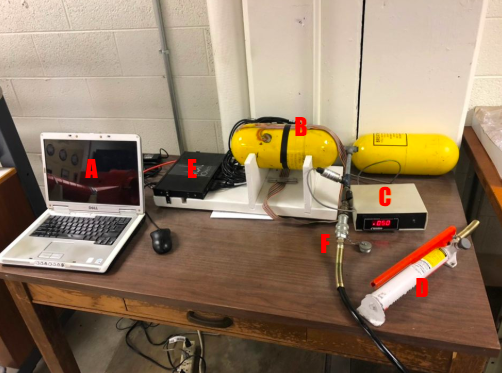
\includegraphics[width=0.9\textwidth]{setup}
	\caption{\textbf{Overhead view of the experiment configuration}}
\end{figure}
Figure 1 shows the full setup for the pressure vessel experiment, with red letters "A-F" to 
label individual components. Letter A represents the Dell Latitude data acquisition machine. The
Excel program was used here to store the measured data. "B" is the MIT-C-5435 oxygen tank, with 
strain rosettes configured on it as shown in \textbf{Figure 2}. "C" is the OMEGA DP-350 pressure
indicator, which retrieves data from "E", the IOtech-6224 strain gage input module, attached to
"F", the OMEGA PX302-500GV pressure transducer. Label D corresponds to the hydraulic hand pump 
that was manually used to control the oxygen tank's internal pressure. 

% Black and white picture of the rosette configurations. Reference to the lab handouts. 
\begin{figure} [H]
	\centering
	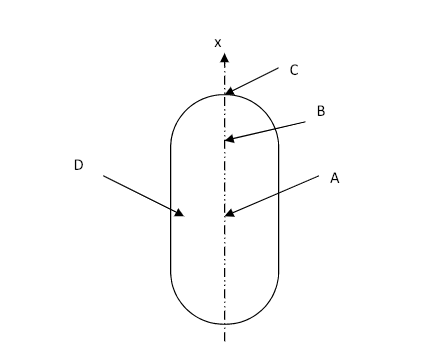
\includegraphics [width=0.4\textwidth]{vessel}
	\caption{\textbf{Overview of the pressure vessel rosette configuration}}
\end{figure} 

% Strain rosette angle configurations. 
\begin{figure} [H]
	\centering
	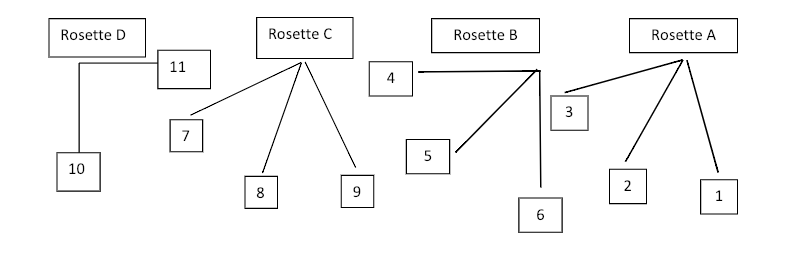
\includegraphics [width=0.9\textwidth]{rosettes}
	\caption{ \textbf{Strain Rosette Angles}}
\end{figure} 
Shown in \textbf{Figure 3} is the configuration of each strain rosette, and \textbf{Figure 4} shows
the angle values which belong to each strain gage. These angles are measured counterclockwise from the 
x axis. Based on the configuration above, certain equivalences can be deduced.

\begin{align}
\epsilon_{4} = \epsilon_{11} \\
\epsilon_{6} = \epsilon_{10} \\ 
2\times\epsilon_{5} = \epsilon_{10} + \epsilon_{11} \\
\epsilon_{7} = \epsilon{_8} = \epsilon_{9} 
\end{align}

\begin{figure} [H]
	\centering
	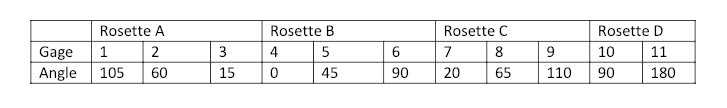
\includegraphics [width=1.0\textwidth]{gage_angles}
	\caption{ \textbf{Strain Rosette Angles}}
\end{figure} 

% Explain each rosette, angles, and possible similarities. 


\paragraph{Test Procedure}
Starting at 0 psig, a hand pump was used to increase the pressure by 50 psig. Once the pressure was set, a mean strain gage was shot selected in the data acquisition program, capturing an instantaneous 
state of mean strain. At 0 psig, theoretically, there should
be zero stress and strain in the vessel. However, strain gages work by measuring micro displacements, and some
minor effects of gravity, age, and physical configuration can cause the voltage at 0 psig to give a value of strain. To
compensate this linear offset, a "normalized" set of data was used, in which every set of data was subtracted from the
zero offset measurement. For example, instead of the strain reading at 100 psig being the raw values pulled from
the data acquisition system, the strain value from 100 psig would be captured, then the difference between the 
baseline value at 0psig would be subtracted from 100 psig, and the resulting value would be the normalized value.  
at 100 psig. All the calculations used the normalized measurements at each pressure increment. This process
was repeated for each strain measurement up to 400 psig. After the ascending measurements were taken, the 
hand pump had its pressure released, and the strain values from 400 psig to 0 psig were taken, in 50 psig 
increments, to determine the descending sets of data. 


\paragraph {Data Reduction Procedure }
The overall flow of data starts at nominal strains, transformed to plane strains, converted  to
principal strains, and finally, through Hooke's law, converted to principal stresses. Once the measured 
principal stresses were obtained, they are  classified as either hoop or axial stresses. For rosettes A, B, and D,
the hoop stress is the larger value, and the axial stress is the smaller value. For rosette C, no hoop stress exists,
because the rosette is placed on the tip of the vessel, there there is no radius. 

\begin{align}
\epsilon_1 = \epsilon_x\cos^{2}\theta_1 + \epsilon_y\sin^{2}\theta_1 + \gamma_{xy}\cos{\theta_1}\sin{\theta_1} \\
\epsilon_2 = \epsilon_x\cos^{2}\theta_2 + \epsilon_y\sin^{2}\theta_2 + \gamma_{xy}\cos{\theta_2}\sin{\theta_2} \\
\epsilon_3 = \epsilon_x\cos^{2}\theta_3 + \epsilon_y\sin^{2}\theta_3 + \gamma_{xy}\cos{\theta_3}\sin{\theta_3} 
\end{align}

These three equations are solved using the matrix multiplication: 
\begin{align}
\begin{bmatrix}
\epsilon_x \\
\epsilon_y \\
\gamma_{xy} \\
\end{bmatrix}
= 
\begin{bmatrix}
   \cos^{2}\theta_1 & \sin^{2}\theta_1 & \cos{\theta_1}\sin{\theta_1}  \\
   \cos^{2}\theta_2 & \sin^{2}\theta_2 & \cos{\theta_2}\sin{\theta_2}  \\
   \cos^{2}\theta_3 & \sin^{2}\theta_3 & \cos{\theta_3}\sin{\theta_3}  \\
\end{bmatrix}^{-1} \times
\begin{bmatrix}
\epsilon_1 \\
\epsilon_2 \\
\epsilon_3 \\
\end{bmatrix}
\end{align}

Once the strain values $\epsilon_x$, $\epsilon_x$, and $\gamma_{xy}$ are calculated, the principal strains
are produced by the equations :
\begin{align}
\epsilon_{p1}, \epsilon_{p2} = \frac{\epsilon_x + \epsilon_y}{2} \pm
\frac{1}{2} \sqrt{ { \frac{\epsilon_x - \epsilon_y}{2}}^2 + {\gamma_{xy}}^2 }
\end{align}


Principal strains lead directly to the principal stresses, given the material properties of the vessel,
in the equation:
\begin{align}
\sigma_{p1} = \frac{E}{1-\nu^2} \big[ \epsilon_{p1} + \nu\epsilon_{p2} \big] \\
\sigma_{p2} = \frac{E}{1-\nu^2} \big[ \epsilon_{p2} + \nu\epsilon_{p1} \big]
\end{align}
	
\paragraph {Data Validity Checking} 
During this experiment, two validity checks were used. As strain measurements were being taken from
the pressure vessel, \textbf{equations 1, 2, 3}, and \textbf{4} were used to check the strain validity. 
Based on the configuration, the values from these four equations should theoretically be the exact same. 
Any differences in the resultant values are due to mechanical error. \\ 

\paragraph{Data Analysis}
After all the measurements were 

% ========== Results ==========
\section{Results and Discussion}\label{conclusions}
\paragraph {Results} 

\begin{table}[H]
  \caption{Normalized Strain data}
  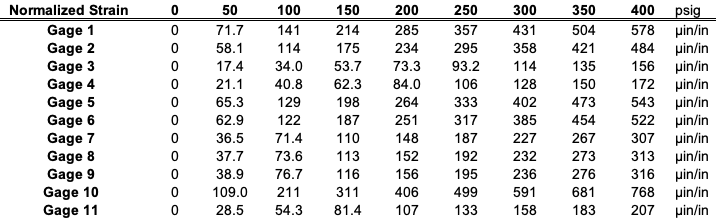
\includegraphics[width=\linewidth]{table_raw_strain}
  \centering
\end{table}

\begin{table}[H]
  \caption{Final calculated stresses using Hooke's law}
  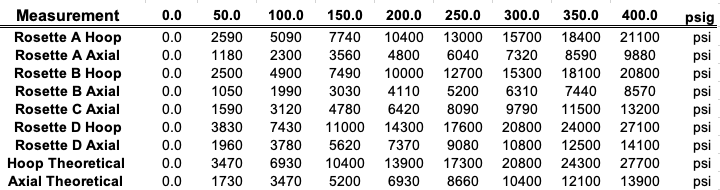
\includegraphics[width=\linewidth]{table_final_stress}
  \centering
\end{table}

\begin{figure} [H]
	\centering
	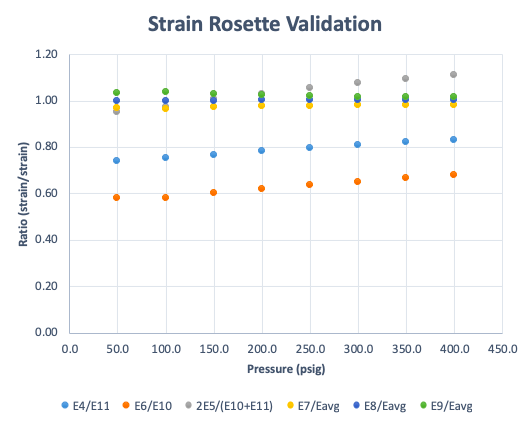
\includegraphics [width=\textwidth]{plot_rosette_validation}
	\caption{ \textbf{Plot showing rosette validation checks}}
\end{figure} 

\begin{table}[H]
  \caption{Strain Rosette Validation Calculations }
  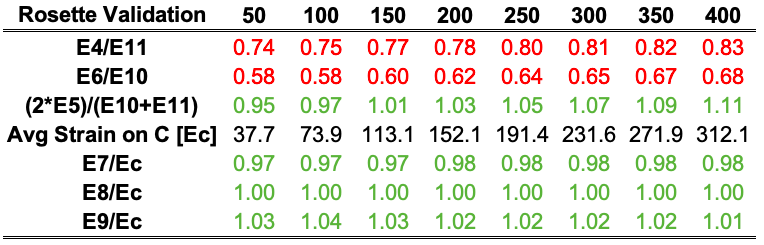
\includegraphics[width=\linewidth]{table_rosette_ratios}
  \centering
\end{table}

\begin{figure} [H]
	\centering
	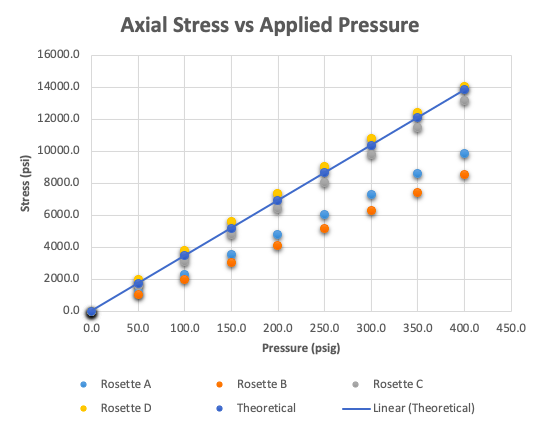
\includegraphics [width=.88\textwidth]{plot_axialvspressure}
	\caption{ \textbf{Calculated Axial stress vs Applied Pressure}}
\end{figure} 

\begin{figure} [H]
	\centering
	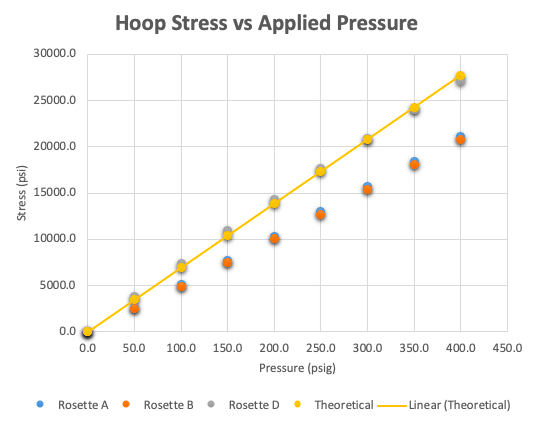
\includegraphics [width=0.87\textwidth]{plot_hoop_measured}
	\caption{ \textbf{Calculated Hoop Stress vs Pressure}}
\end{figure} 

\begin{figure} [H]
	\centering
	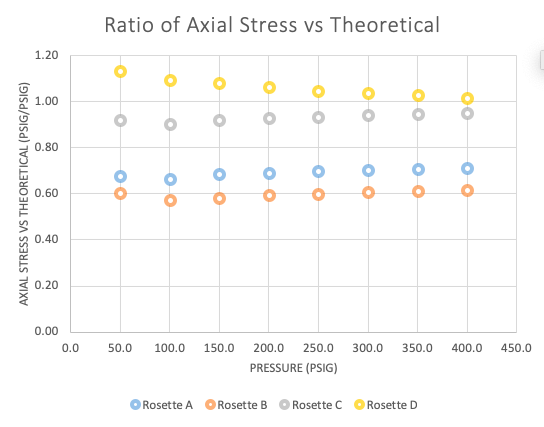
\includegraphics [width=1.0\textwidth]{plot_axialvstheor}
	\caption{ \textbf{Ratio of Rosette Axial Stress vs Theoretical Stress}}
\end{figure} 

\begin{table}[H]
  \caption{Ratio of calculated axial stress to theoretical stress}
  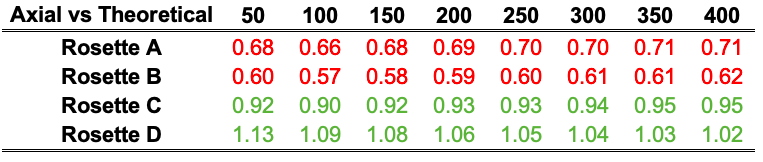
\includegraphics[width=\linewidth]{table_axial_theory}
  \centering
\end{table}

\begin{figure} [H]
	\centering
	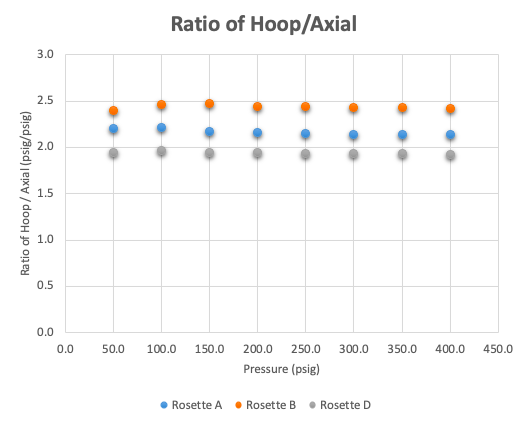
\includegraphics [width=1.0\textwidth]{plot_hoop_vs_axial}
	\caption{ \textbf{Ratio of Hoop vs Axial stress for rosettes A B D }}
\end{figure} 

\begin{table}[H]
  \caption{Table of Hoop vs Axial stress per rosette}
  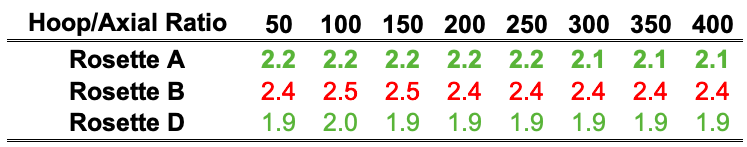
\includegraphics[width=\linewidth]{table_hoop_axial}
  \centering
\end{table}

\begin{figure} [H]
	\centering
	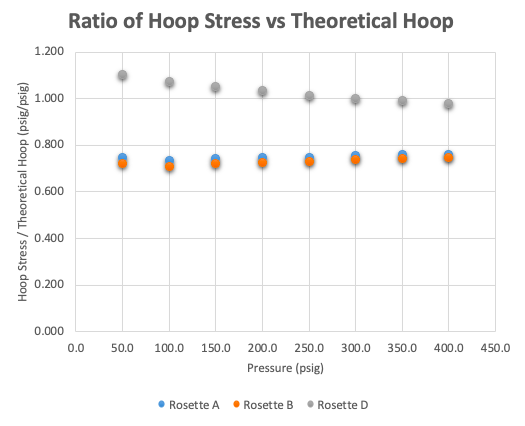
\includegraphics [width=1.0\textwidth]{plot_hoop_vs_theoretical_ratio}
	\caption{ \textbf{ Ratio of calculated Hoop stress vs theoretical hoop stress }}
\end{figure} 

\begin{table}[H]
  \caption{Table showing Hoop Stress vs Theoretical Stress for A,B, and D }
  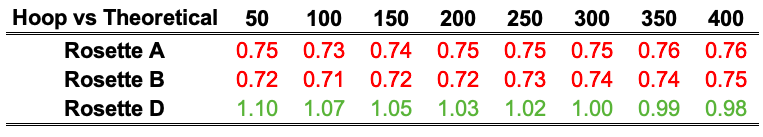
\includegraphics[width=\linewidth]{table_hoop_theoretical}
  \centering
\end{table}

% ========== Discussion section  ==========
\section {Conclusions and Recommendations}



% ========== References ==========
\section {References}


% ========== Appendices ==========
\section {Appendices}

\end{document}
